\chapter{Design}
\label{ch:design}
\section{Introduction}
This section describes the design process of the project. There are a number of diagrams, tables, and methodologies used while designing the system. This phase is key to implementing a successful system, as it forms the basis for the implementation of the project, ensuring that the requirements of the system are met in a timely and effective manner.

\section{Technologies}
This section outlines the technologies that will be used for the project, and gives a justification for why each technology will be used. This includes programming languages, web frameworks, and libraries.

\subsection{Programming Languages}
\label{sec:lang}
Based on the research in Chapter~\ref{ch:lit}, there are a number of candidates for developing a chatbot system. Table~\ref{tab:lang} summarises the main features of each, and how they might be effective for this project.

\begin{table}[h]
	\centering
	\begin{tabularx}{\textwidth}{{@{}lXXX@{}}}
		\toprule
		& Java & Python & Ruby on Rails \\
		\midrule
		Description 
			& Popular object-oriented language used in many enterprise solutions.
			& A well-established language in data science and machine learning communities.
			& Interpreted language commonly combined with Rails in web applications. \\
		Advantages
			& Popular language with a large community.
			
			Java Virtual Machine (JVM) allows for integrated cross-platform support.
			
			& Abundant range of libraries for machine learning.
			
			Widely used in artificial intelligence applications.
			
			& Inherently web-based, Ruby on Rails design principles such as `Convention over Configuration' allow for
			  rapid development of web applications. \\
  		Disadvantages
  			& Web-based applications require additional libraries.
  			& Not inherently web-based, although frameworks exist such as Django \cite{django2020}.
  			& Less maintainable than other web frameworks \cite{plekhanova2009evaluating}.
  			\\
		Examples
			& Corpus-training an ALICE chatbot by \citet{shawar2011corpus}.
			& Chatbot techniques survey by \citet{abdul2015survey}.
			& Shopping chatbot by \citet{horzyk2009intelligent}.
			\\
  
				
	\end{tabularx}
	\caption{Comparison of programming language candidates.}
	\label{tab:lang}
\end{table}

Given the scale and scope of this project, many of the nuances and disadvantages seen in Section~\ref{sec:langreview} are irrelevant to a smaller project such as this. There appears to be libraries and frameworks in most languages that will allow the development of this system. As such, personal preference can also be considered in the choice, such as familiarity and confidence with given languages and libraries. Therefore, the project will be developed in Java, because of personal experience and familiarity with the language.


\subsection{Web Frameworks}
In the case of Java, there are several web frameworks that can be used to handle webpage design, routing, and configuration.

\subsection{Chatbot Model}


\subsection{Libraries and Tools}
This section describes the libraries and tools required to implement the chatbot system in Java. Table~ describes each library and its function.

Table here

\newpage
\section{Architecture}
\subsection{System Design}
The overall implementation will have a number of interacting modules in order to accept user input, perform processing, and generate an output based on information from the DBPedia database. Figure~\ref{fig:design_system} provides a visual representation of this. The user input is matched against the set of chatbot AIML patterns, which determine the query requirements. The query is then built based on the values provided by the user and set by the AIML system. The SPARQL query is executed against the DBPedia live database, and the results are received and processed by the response builder. The response is displayed to the user. Although the architecture is simple, many considerations have to be made by each module, especially when dealing with users who may ask a range of questions in several different ways.

\begin{figure}[h]
	\begin{center}
		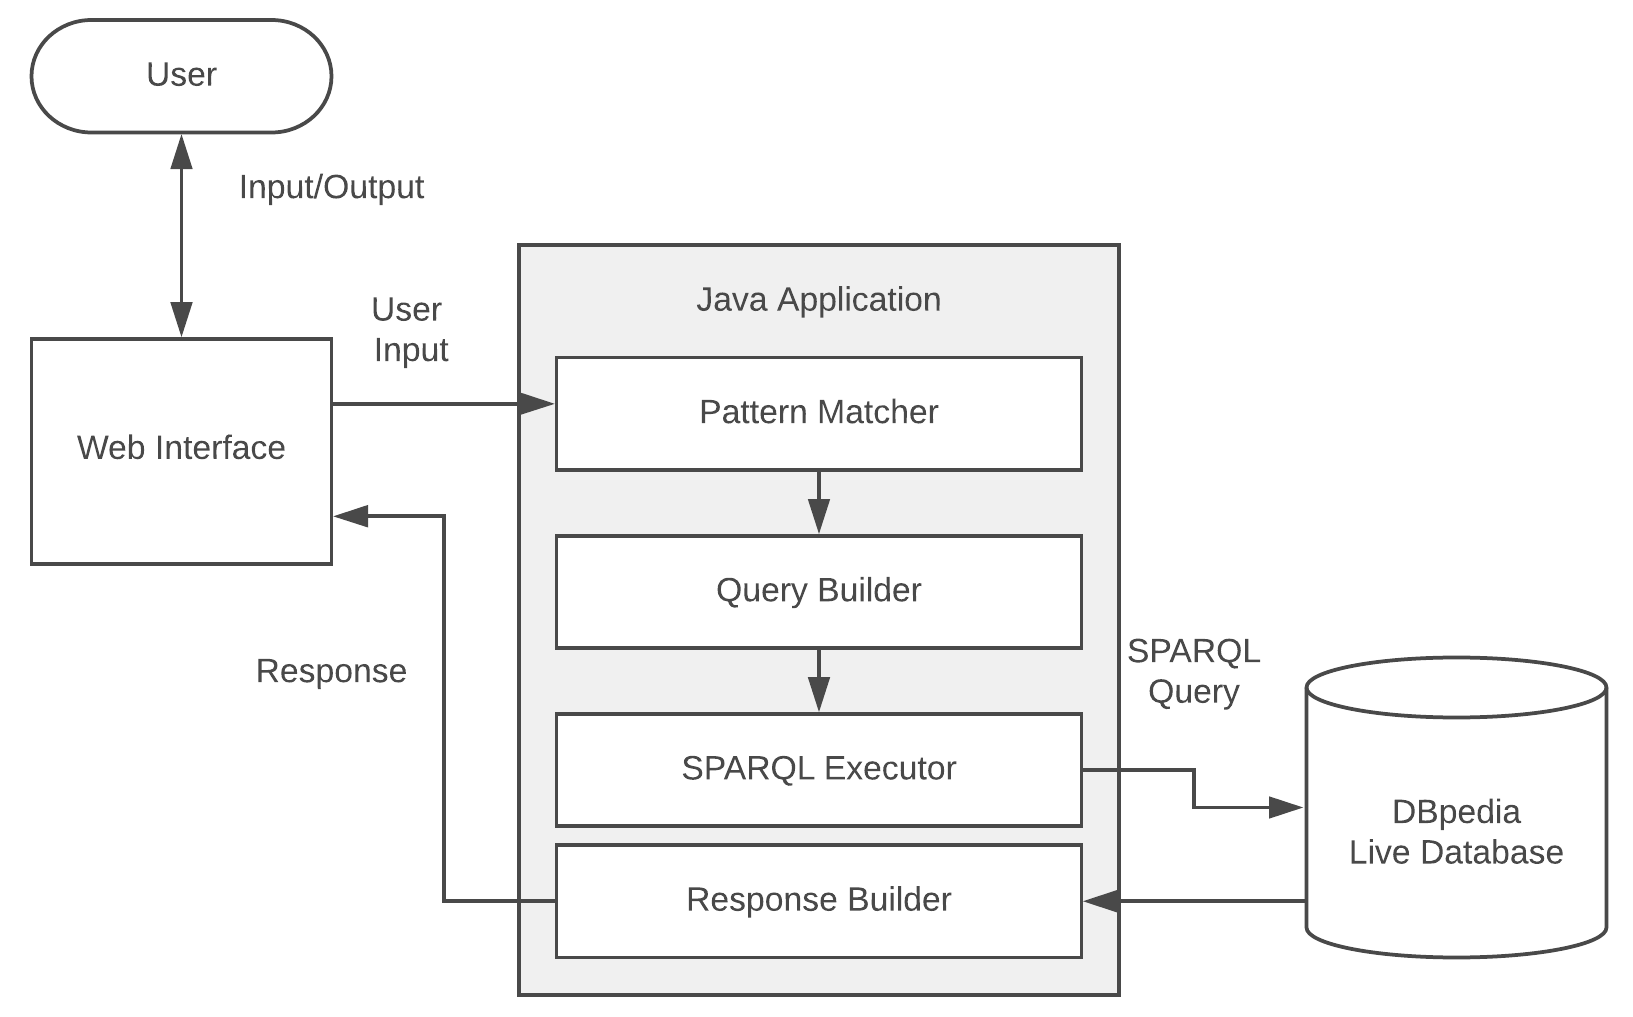
\includegraphics[width=\textwidth]{design_system}
	\end{center}
	\caption{Overview of architecture of the system.}
	\label{fig:design_system}
\end{figure}

\newpage
\subsection{Activity}
Figure~\ref{fig:design_activity} shows the flow of events through the system, from the user input to the resulting output. The activity starts in the web page, where the user inputs a query and posts it to the system. Processing of this query is performed by the Java application, which generates a query and sends it to the SPARQL endpoint. The response is received by the application, and processed into a response which is displayed in the web page.

\begin{figure}[h]
	\begin{center}
		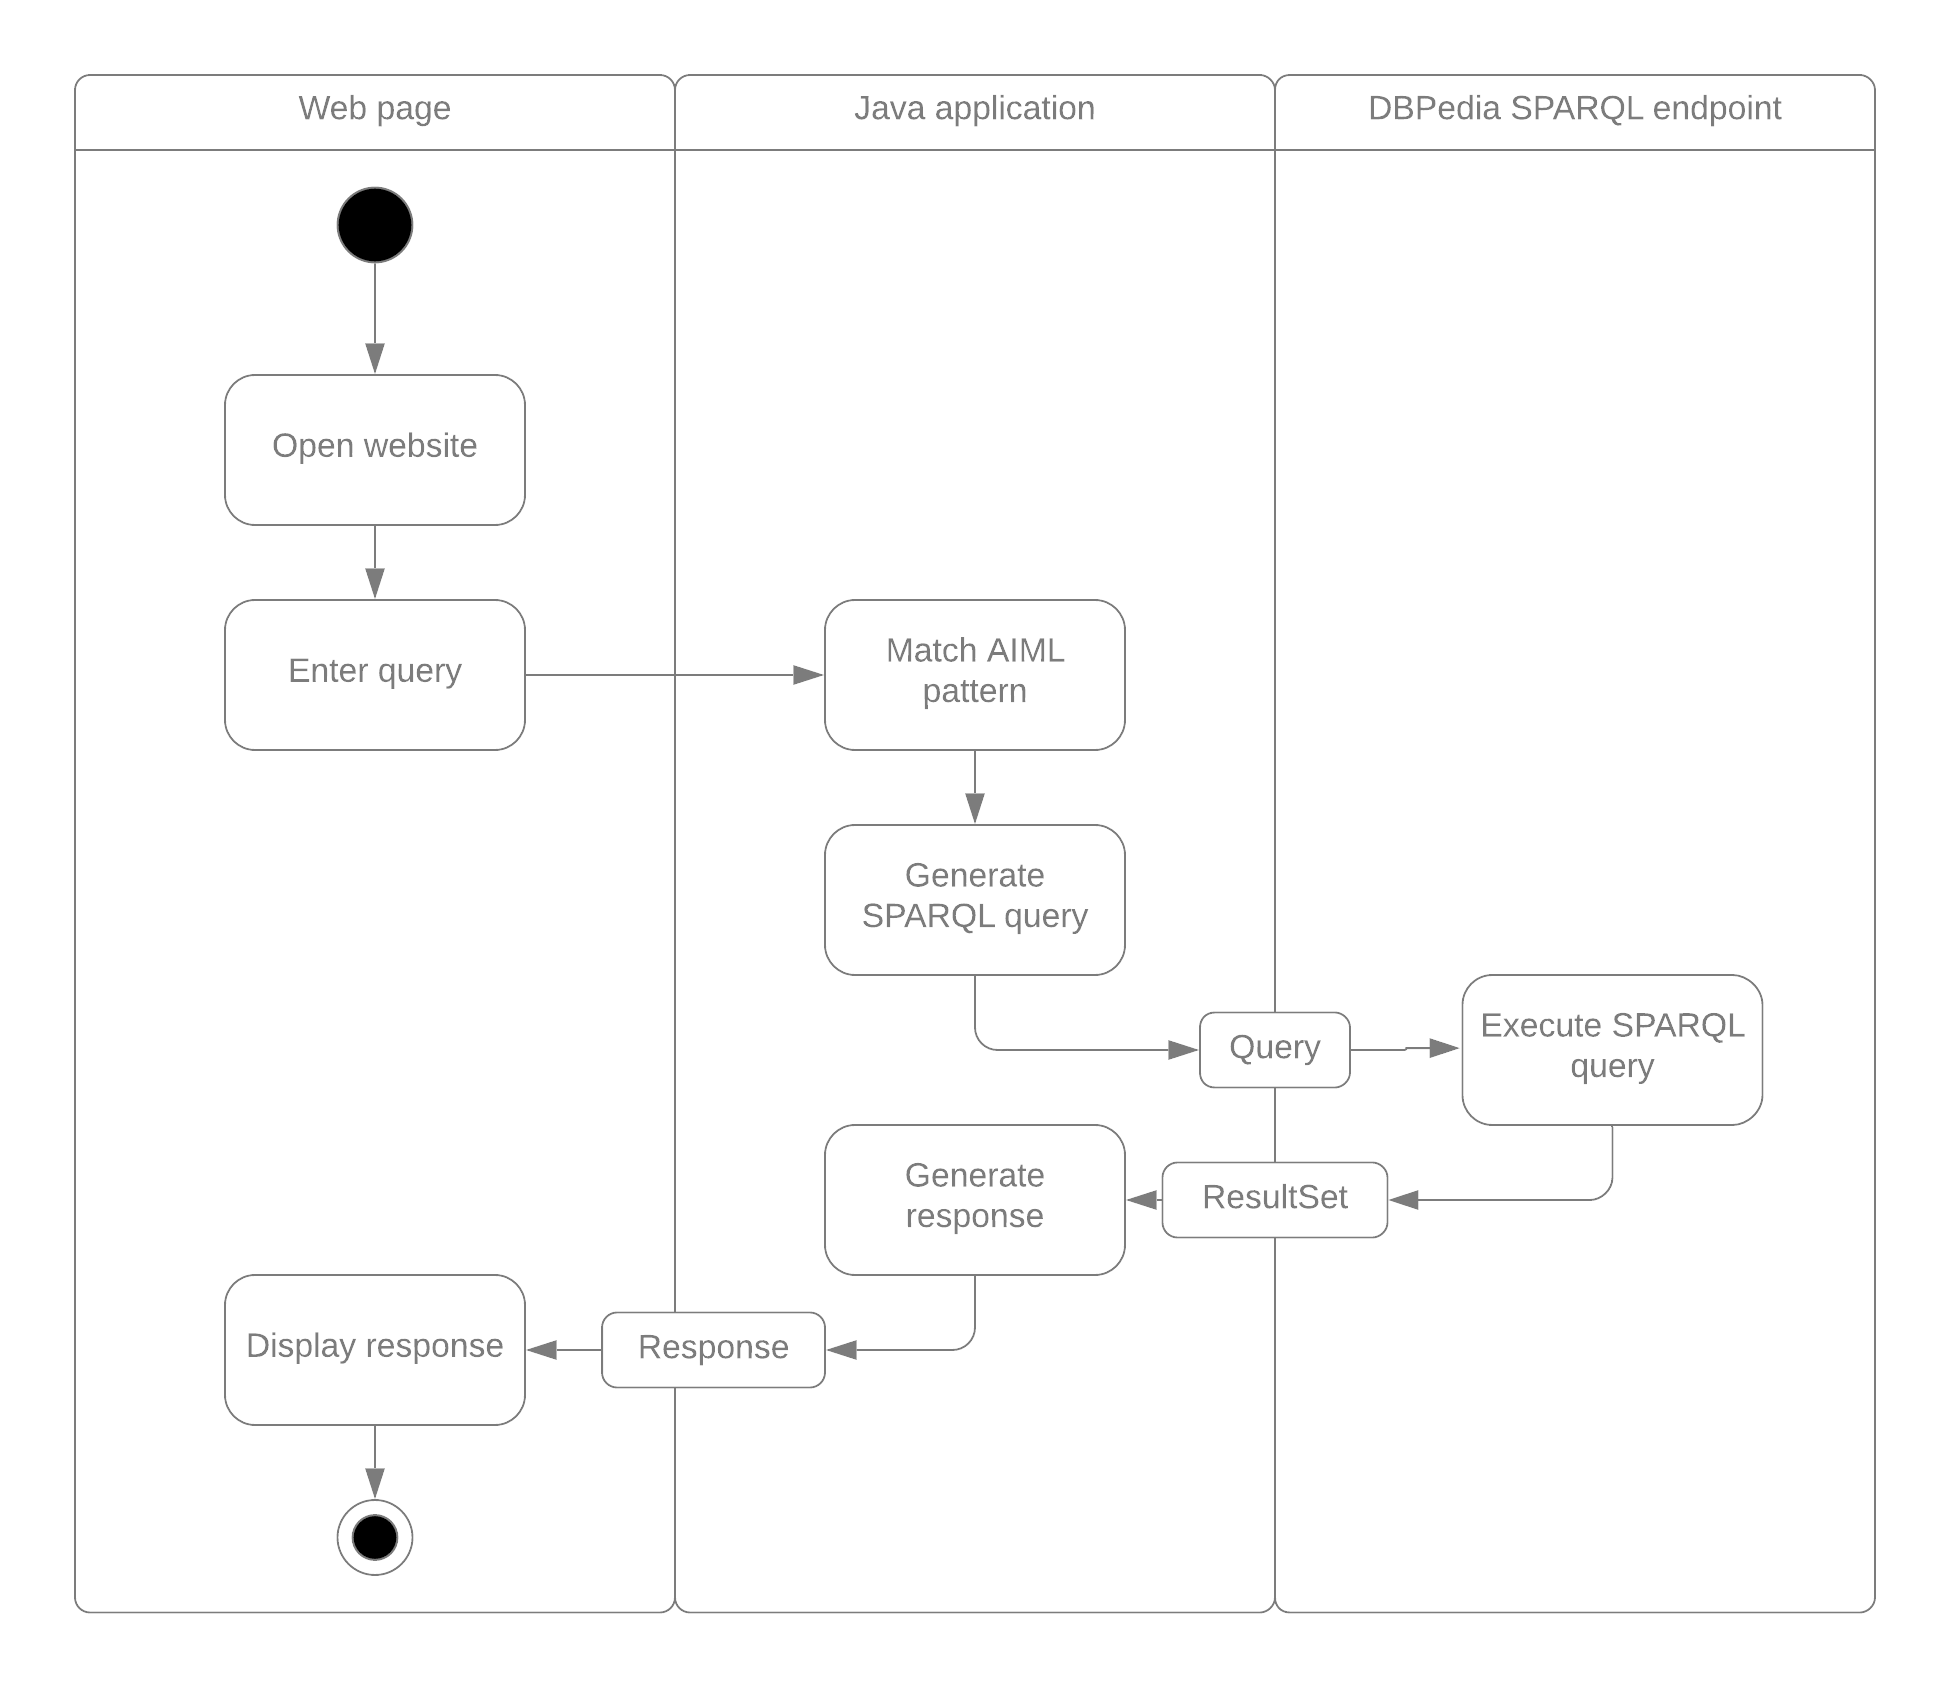
\includegraphics[width=\textwidth]{design_activity}
	\end{center}
	\caption{UML Activity diagram.}
	\label{fig:design_activity}
\end{figure}

\section{Conversation Flowchart}
One of the requirements of the system is maintaining the context of the conversation through multiple lines of dialogue. This means that if a user has asked a question about a person -- ``Who is Alan Turing?'' --, they can then ask follow-up questions -- ``What is he known for?''. This prevents the user having to repeat the subject of each question, allowing for a more natural conversation flow. Figure~\ref{fig:flowchart} shows a flowchart for this conversation flow, and how the chatbot will set and maintain the conversation context.

\begin{figure}[h]
	\begin{center}
		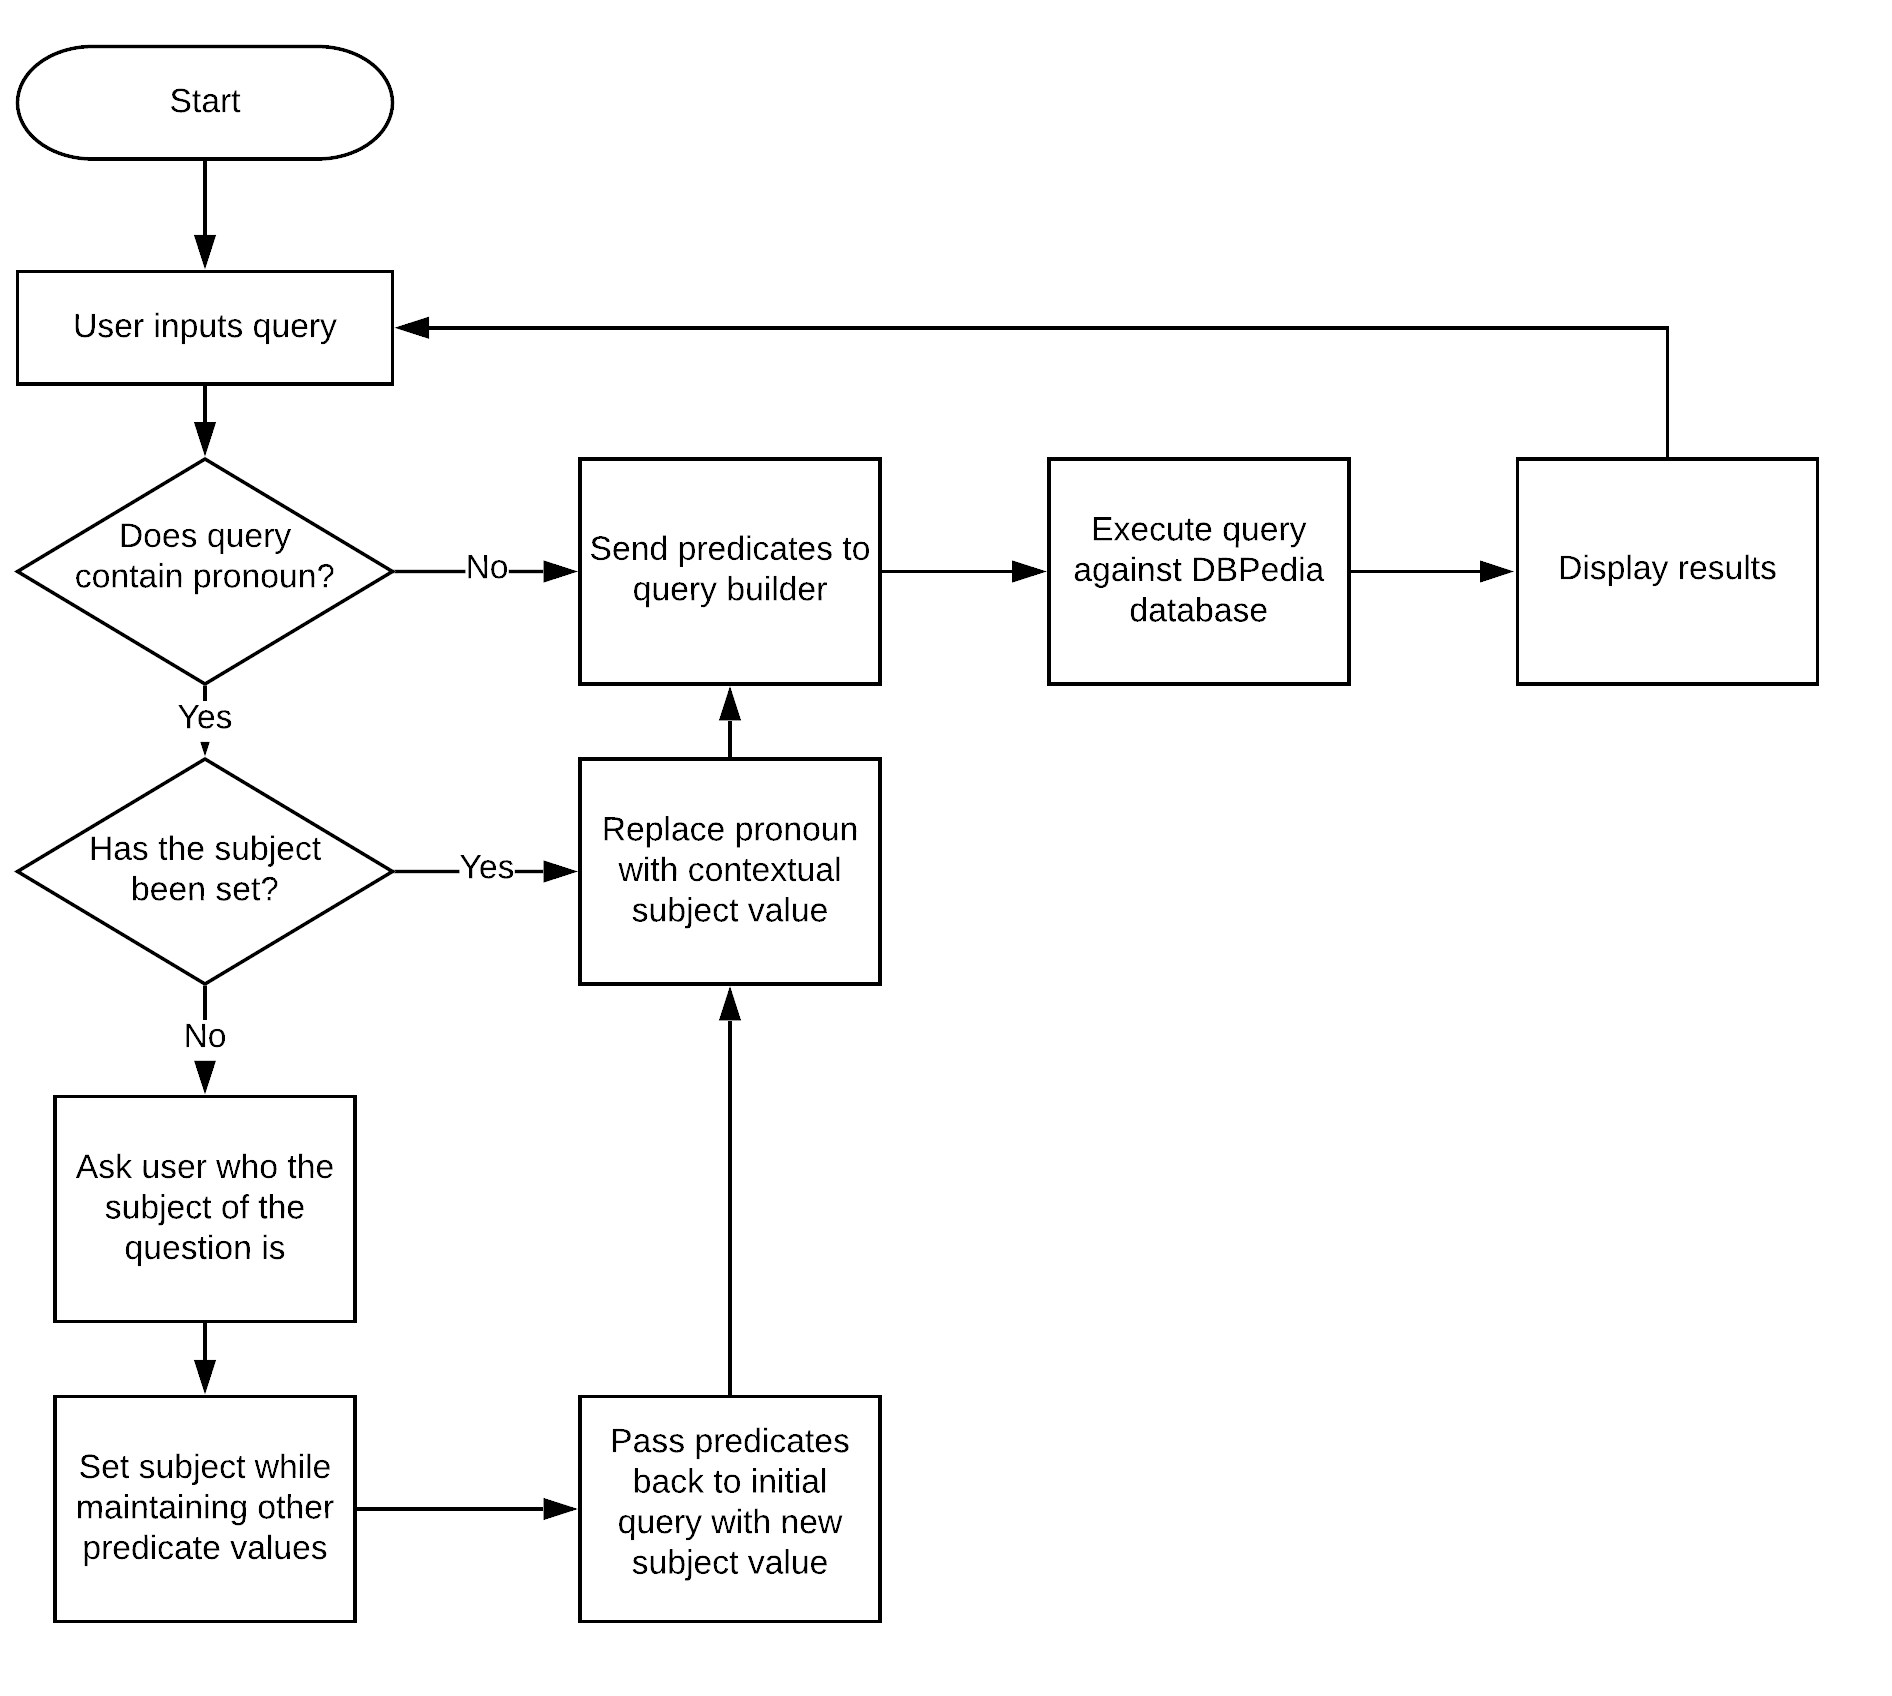
\includegraphics[width=\textwidth]{flowchart}
	\end{center}
	\caption{Conversation flowchart diagram.}
	\label{fig:flowchart}
\end{figure}

\section{Class Diagram}
Class diagram
\begin{figure}[h]
	\begin{center}
		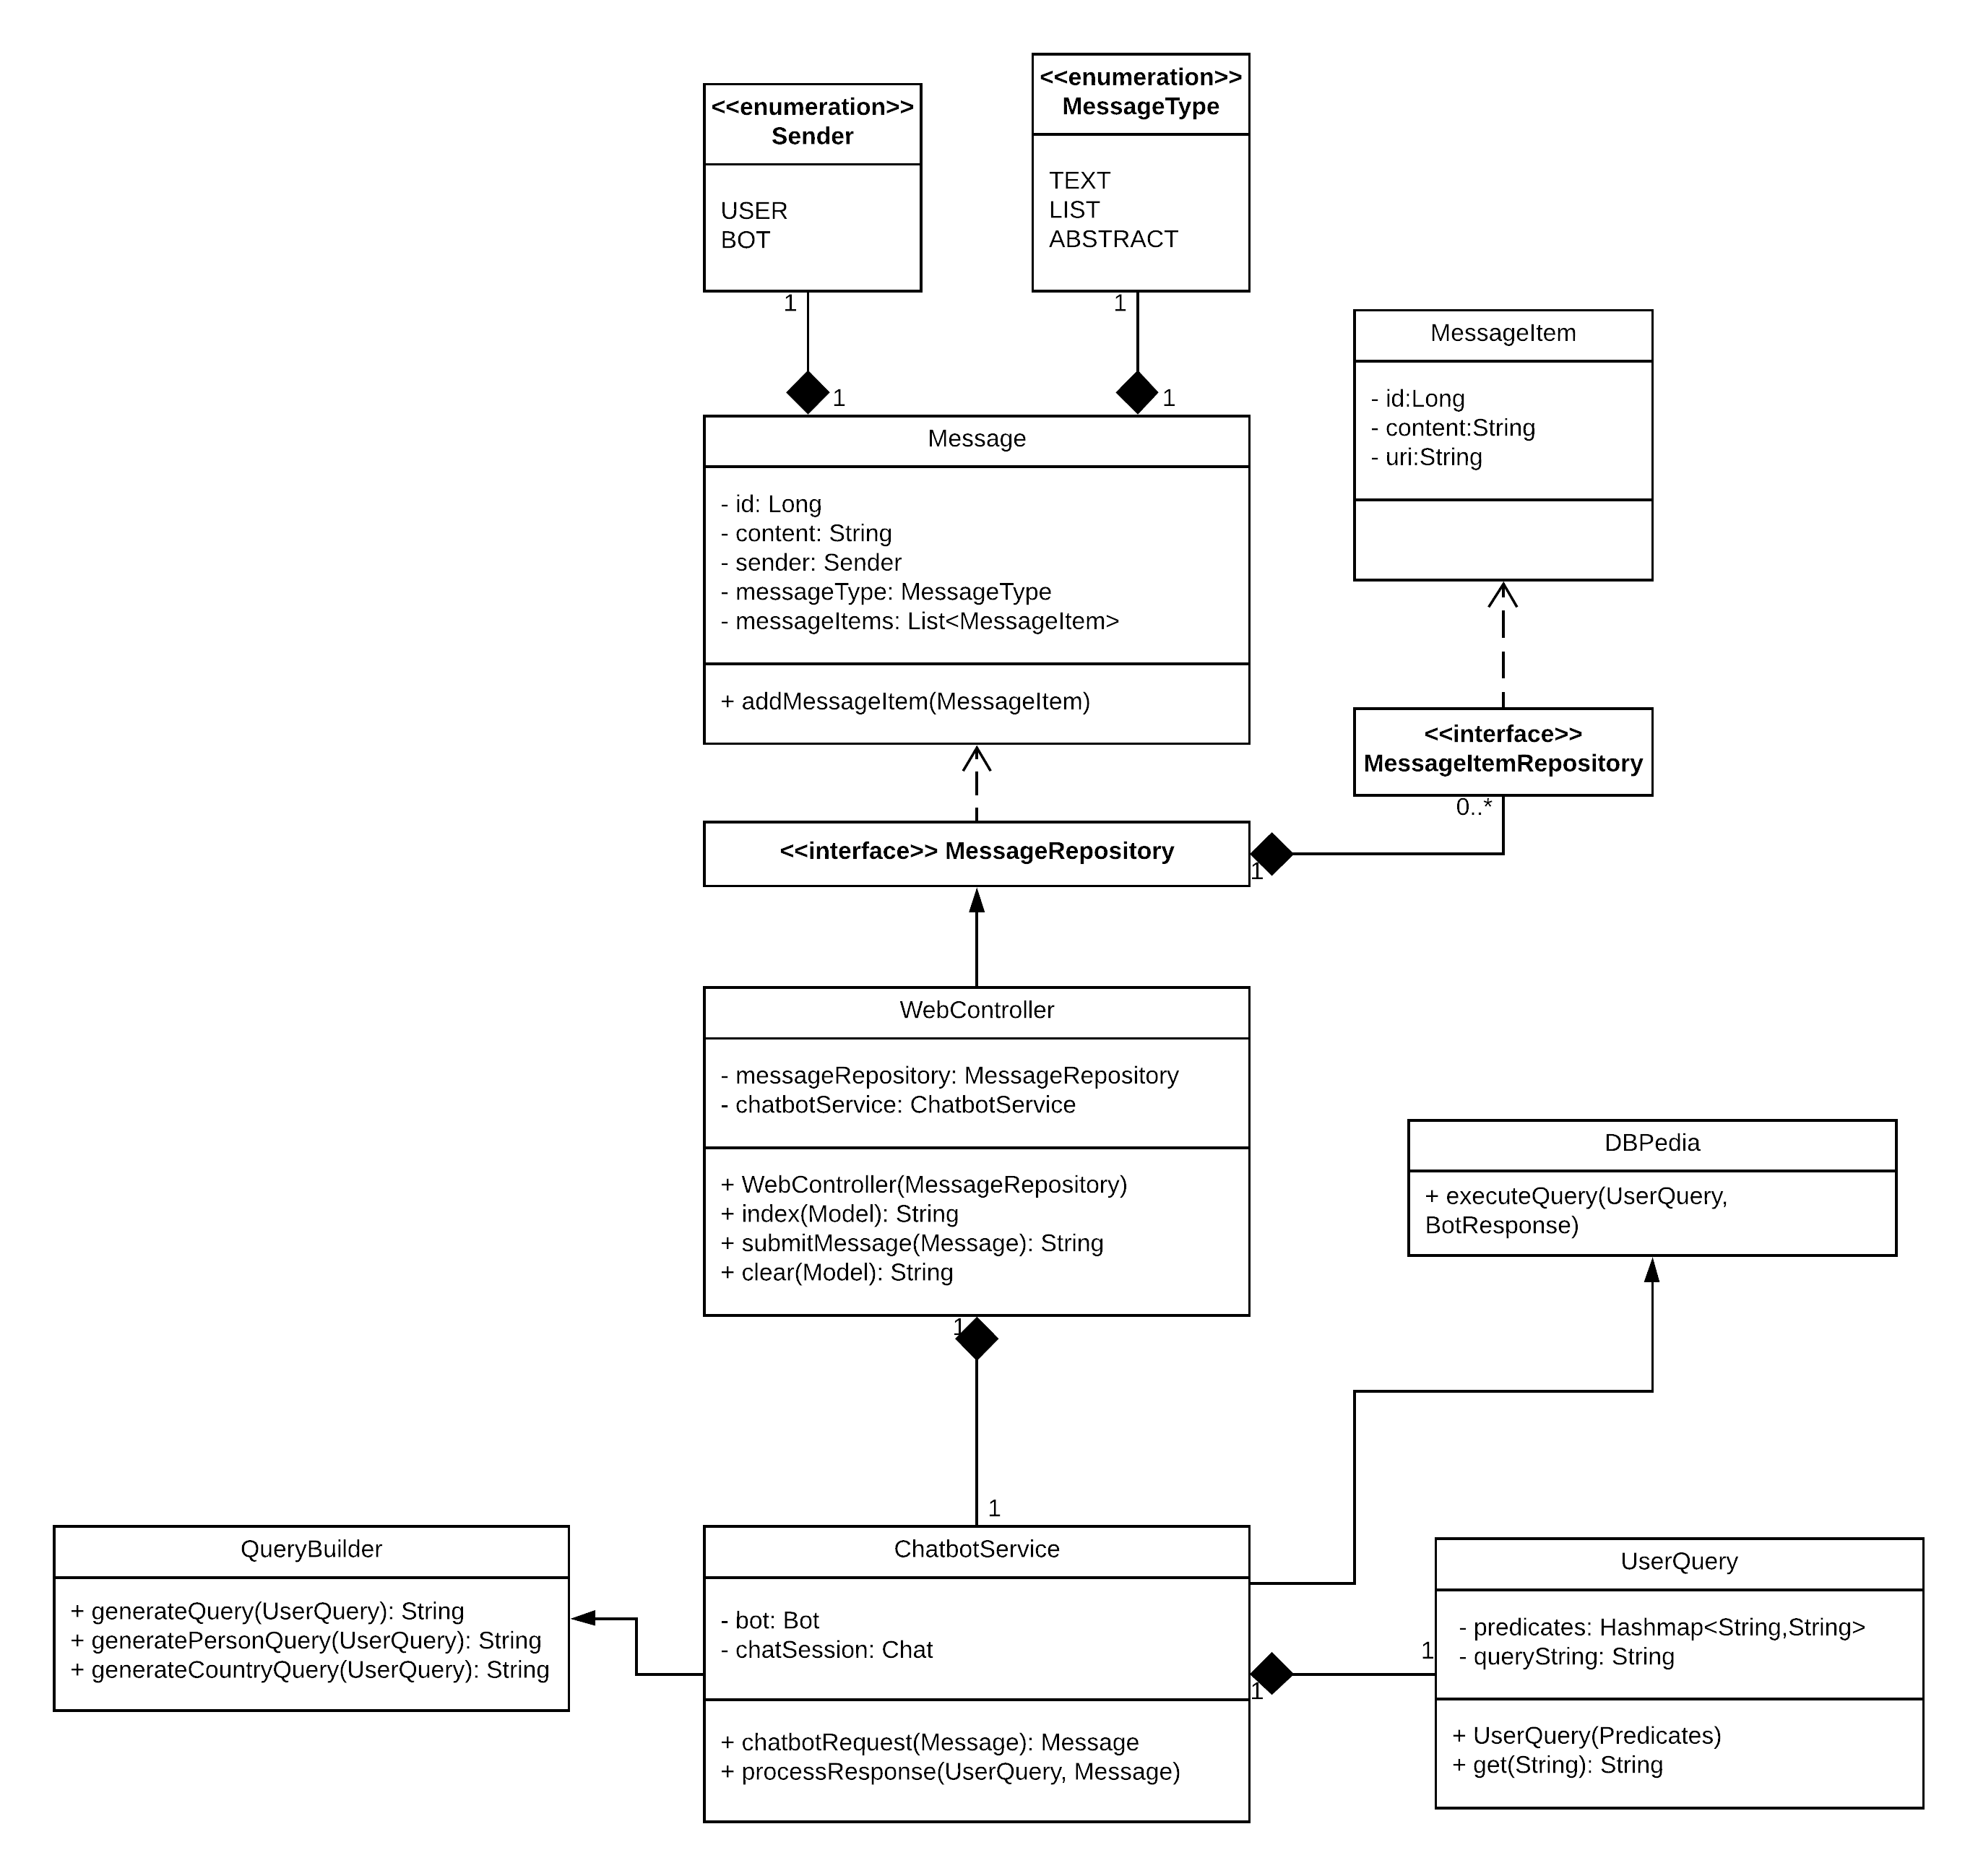
\includegraphics[width=\textwidth]{class_diag}
	\end{center}
	\caption{UML Class diagram.}
	\label{fig:class_diagram}
\end{figure}

\newpage
\section{User Interface}
The proposed system will be a web application for a number of reasons. Firstly, it will allow testers to easily access the application without having to download any files. It also allows for easy customisation using HTML and CSS. The alternative would be a text-based user interface (TUI), which would require less configuration, but will be limited in terms of rendering images, links, and other elements. It will be beneficial to use a TUI during development, as this would allow the system to be built and debugged quickly. Figure~\ref{fig:design_ui} shows the expected web interface design for the system.

\begin{figure}[h]
	\begin{center}
		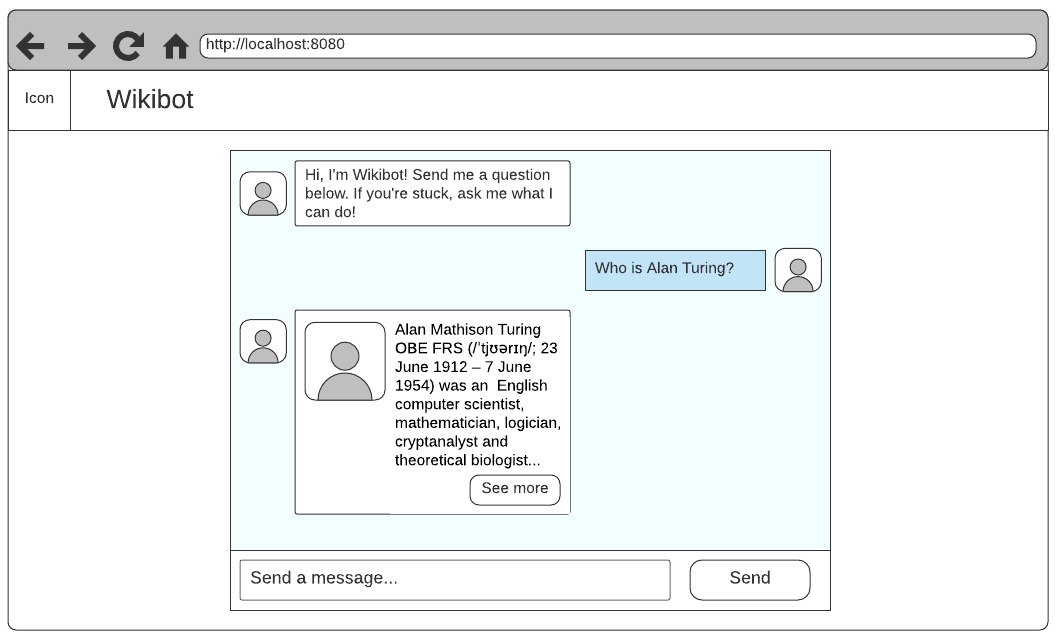
\includegraphics[width=\textwidth]{design_ui}
	\end{center}
	\caption{Web UI interface design.}
	\label{fig:design_ui}
\end{figure}

\section{Data}